\section{Bell Inequalities}
In this section we will cover only one inequality, the CHSH inequality which was first proposed in 1969. Let us first start with experimental setting, 

\begin{figure}[h!]
\centering
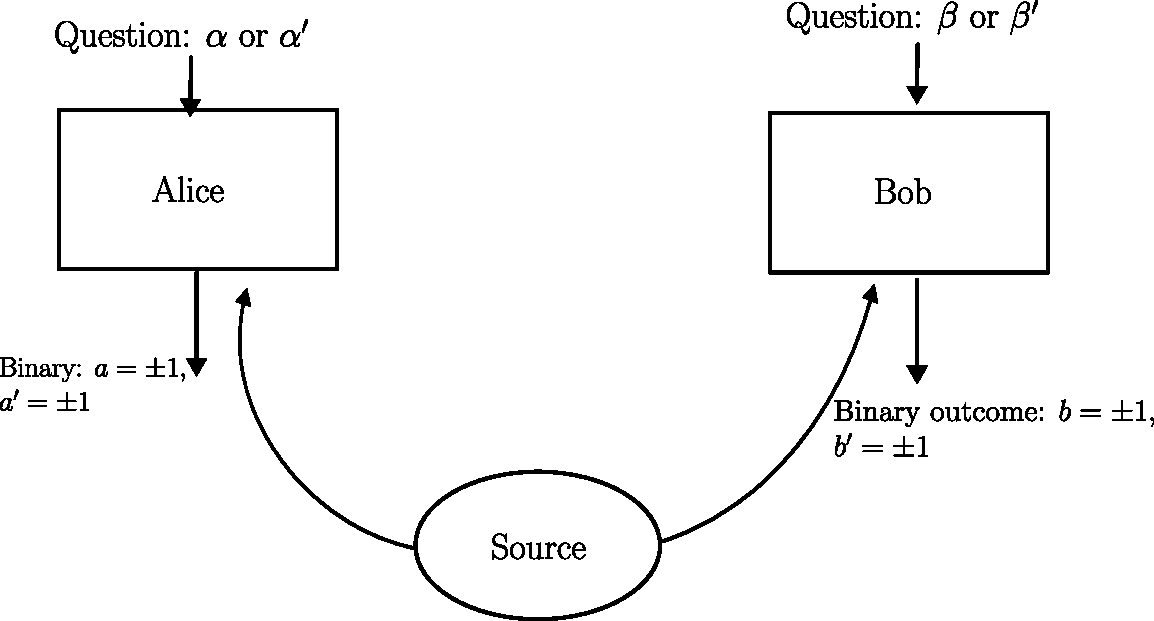
\includegraphics[width=0.6\textwidth]{figures/2026-10-14.pdf}
\caption{Experimental Setting}
\end{figure}

Alice does measurements with the following basis :
\begin{align*} 
	 &\begin{cases}
	 	\ket{\alpha} = \cos \alpha \ket{ 0} + \sin \alpha \ket{ 1}\\
		\ket{\alpha_\perp} = -\sin \alpha \ket{0} + \cos \alpha \ket{1}
	 \end{cases} \\
	 &\begin{cases}
	 	\ket{\alpha'}, \ket{\alpha_\perp '}
	 \end{cases} 
\end{align*}
The outcome of those measurements is given as random variables
\begin{align*} 
	a = \pm 1\\
	a' = \pm 1
\end{align*}
Bob also measures with a basis 
\begin{align*} 
	\left\{\ket{\beta}, \ket{\beta_\perp}\right\} \\
	\left\{\ket{\beta'}, \ket{\beta_\perp'}\right\}
\end{align*}
With the outcome of the measurements being also random variables 
\begin{align*} 
	b = \pm 1\\
	b' = \pm 1
\end{align*}
Which gives four possibilities 
\begin{align*} 
	\left(\alpha, \beta\right) &\to \left(a, b\right) \\
	\left(\alpha', \beta\right) &\to \left(a', b\right)\\
	\left(\alpha, \beta'\right) &\to \left(a,b'\right)\\
	\left(\alpha', \beta'\right) &\to \left(a', b'\right)
\end{align*}
Then after this they collect their strings A and B and communicate and exchange their results. After having collected everything, they will compute the \important{correlation coefficient} which is given as (knowing $N_1 \approx N_2 \approx N_3 \approx N_4 \approx \frac{N}{4}$)
\begin{align*} 
	X^{\text{experimental}} = \frac{1}{N_1} \sum_{i_1 : \left(\alpha, \beta\right)} a_{i_1} b_{i_1} + \frac{1}{N_2} \sum_{i_2 : \left(\alpha, \beta'\right)}a_{i_2}b_{i_2}' - \frac{1}{N_3} \sum_{i_3 : \left(\alpha' ,\beta\right)} a_{i_3}'b_{i_3} + \frac{1}{N_4} \sum_{i_4 : \left(\alpha', \beta'\right)} a_{i_4}'b_{i_4}'
\end{align*} 

\begin{parag}{Theoretical prediction}
    The theoretical prediction of our experiment is given as 
	\begin{align*} 
		X^{\text{theory}} = \mathbb{E}_{\alpha \beta}\left(ab\right) + \mathbb{E}_{\alpha \beta'}\left(a b'\right) - \mathbb{E}_{\alpha' \beta}\left(a' b\right) + \mathbb{E}_{\alpha' \beta'}\left(a' b'\right)
	\end{align*}
	To be able to compute this we need to introduce the hidden variable local theory in order to give a view point of a '\textit{classical physicist}'.\\
	$ $\\
	What we are saying is that the outcome of a measurement of $\alpha$ into $a$ is given by the probability 
	\begin{align*} 
		P_A\left(a | \alpha, \lambda\right) 
	\end{align*}
	Where $\lambda$ is a collection of hidden variables, meaning that the outcome distribution is determined by $\lambda$ and the setting $\alpha$. What's important here is also the '\textit{local}' word, the result of $a$ does not depend on $\beta$, the experiment of Alice is not influenced by any other factor.\\
	$ $\\
	The same mechanism works with Bob giving
	\begin{align*} 
		P_B\left(b | \beta, \lambda\right) 
	\end{align*}
	\begin{center}
	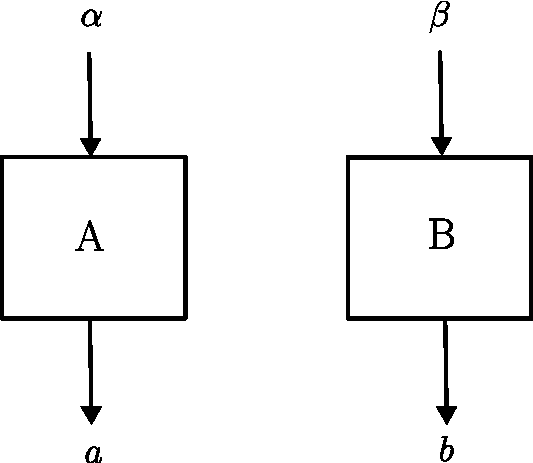
\includegraphics[width=0.4\textwidth]{figures/2026-10-14_1.pdf}
	\end{center}
	Which can be formalized as 
	\begin{align*} 
		P\left(a, b| \alpha, \beta, \lambda\right) = P_A\left(a| \alpha, \lambda\right)P_B\left(b|\beta, \lambda\right) 
	\end{align*}
	We also assume that the hidden variables are distributed according to some distribution $h\left(\lambda\right)$ which does \important{not} depend on the settings $\alpha, \beta$ (\important{measurement independence} or '\textit{free choice}'). This is the third standard assumption alongside locality and realism (hidden variables): without it, we could not use the same $h\left(\lambda\right)$ in all four expectations.
\end{parag}

\begin{theoreme}{CHSH inequality (Bell inequality)}
	\begin{align*} 
		-2 \leq X^{\text{LHV theory}}  \leq 2
	\end{align*}
\end{theoreme}
\begin{proof}
    Let us first try to compute $\mathbb{E}_{\alpha, \beta}\left(ab\right)$. To do so we first need to compute the conditional over $\lambda$ times the probability of $\lambda$ which implies integrating over $\lambda$:
	\begin{align*} 
		\mathbb{E}_{\alpha, \beta}\left(ab\right) &= \sum_{a, b =  \pm 1}ab \int d \lambda P\left(a, b| \alpha, \beta, \lambda\right)h\left(\lambda\right) \\
												  &= \sum_{a, b = \pm 1} ab \int d \lambda P_A\left(a | \alpha, \lambda\right) P_B\left(b | \beta, \lambda\right)h\left(\lambda\right)
	\end{align*}
	Note that $h\left(\lambda\right) \geq 0$ and $\int h\left(\lambda\right)d \lambda = 1$, also adding the probability distribution of $a'$ and $b'$ (which shouldn't change anything as their sums are $1$).
	\begin{align*} 
		= \sum_{a, a', b, b' \in \left\{\pm 1\right\}} ab \int d \lambda P_A\left(a' | \alpha', \lambda\right) P_A\left(a | \alpha,  \lambda\right)P_B \left(b' | \beta', \lambda\right) P_B\left(b | \beta, \lambda\right) h\left(\lambda\right)
	\end{align*}
	Let us now define 
	\begin{align*} 
		Q\left(a, a', b, b'| \alpha, \alpha', \beta, \beta'\right) = \int d \lambda P_A\left(a| \alpha, \lambda\right) P_A\left(a'|\alpha', \lambda\right) P_B \left(b| \beta, \lambda\right) P_B\left(b'| \beta', \lambda\right) h\left(\lambda\right) 
	\end{align*}
	Let us simplify the notation by removing the conditional for convenience (they are still there), which implies that our expected value $\mathbb{E}_{\alpha \beta}\left(ab\right)$ can be rewritten as 
	\begin{align*} 
		\mathbb{E}_{\alpha, \beta}\left(ab\right) &=  \sum_{a, a', b, b'} ab\, Q\left(a, a', b, b'\right)
	\end{align*}
	The key idea is that $Q$ is a genuine joint probability distribution over all four outcomes: $Q \geq 0$ and $\sum_{a, a', b, b'} Q\left(a, a', b, b'\right) = 1$. Locality plus hidden variables guarantees that such a joint distribution exists, even though $a$ and $a'$ (or $b$ and $b'$) can never be measured together. This is the whole content of the theorem.
	Which means that our random variable can be rewritten as 
	\begin{align*} 
		X^{\text{LHV theory}} &=  \sum_{a, a', b, b'}Q\left(a, a', b, b'\right)\left[ab + ab' - a'b + a'b'\right]\\
		&= \sum_{a, a', b, b'}Q\left(a, a', b, b'\right)\left[a\left(b + b'\right) + a'\left(b' - b\right)\right]
	\end{align*}
	Notice here that all random variables here are binary which means that $\left(b + b'\right)$ can either be $0, 2$ or $-2$. Notice now that the case $b = b'$ gives $2ab + 0 = \pm 2$, and if $b \neq b'$ (e.g.\ $b = 1, b' = -1$) we get $0 - 2a' = \pm 2$. We can convince ourselves that the result of the $\left[\cdot \right] = \pm 2$. Therefore
	\begin{align*} 
		\left|X^{\text{LHV theory}}\right| \leq \sum_{a, a', b, b'} Q\left(a, a', b, b'\right) \left|\left[\cdot\right]\right| = 2 \sum_{a, a', b, b'} Q\left(a, a', b, b'\right) = 2
	\end{align*}
\end{proof}

 We can show that the hidden variable local theory cannot be applied to quantum mechanics! Meaning that the joint distribution of our two states here cannot be factorized into a product of two probability distributions. Intuitively, this is related to Bell states or more generally entangled states (which cannot be factorized into tensor products). Concretely, we have that for EPR Bell pairs distributed by some
\begin{align*} 
	\lambda \leftrightarrow \ket{B_{00}}  = \frac{1}{\sqrt{2}}\left(\ket{0_A0_B} + \ket{1_A1_B}\right)
\end{align*}
We find that 
\begin{align*} 
	\max_{\alpha, \beta, \alpha', \beta'} X^{\text{QM theory}}\left(\alpha, \beta, \alpha', \beta'\right) = 2 \sqrt{2} 
\end{align*}

Which therefore implies that quantum mechanics cannot be represented using the hidden variable local theory, meaning technically that quantum mechanics is \important{non-local}.



\begin{parag}{Quantum prediction for Bell pairs (EPR pairs)}
    Let us now look at the same '\textit{experiment}' but with Bell pairs, we have a source of qubits for $i = 1, \ldots, N$ with a distribution $\ket{B_{00}}= \frac{1}{\sqrt{2}}\left(\ket{0}_A \otimes \ket{0}_B + \ket{1}_A \otimes \ket{1}_B\right)$ with $A$ and $B$ observables defined as 
	\begin{align*} 
		A &=  \left(+1\right) \ket{\alpha}\bra{\alpha} + \left(-1\right) \ket{\alpha_\perp}\bra{\alpha_\perp}\\
		A'&= \left(+1\right)\ket{\alpha'}\bra{\alpha'} + \left(-1\right) \ket{\alpha_\perp'}\bra{\alpha_\perp'}
	\end{align*}
	And the same for Bob 
	\begin{align*} 
		B &=  \left(+1\right) \ket{\beta}\bra{\beta} + \left(-1\right) \ket{\beta_\perp}\bra{\beta_\perp}\\
		B'&= \left(+1\right)\ket{\beta'}\bra{\beta'} + \left(-1\right) \ket{\beta_\perp'}\bra{\beta_\perp'}
	\end{align*}
	Our goal is to compute the expected value as in the classical case which is given as 
	\begin{align*} 
		X^{\text{QM theory}}  &= \bra{B_{00}}A \otimes B \ket{B_{00}} + \bra{B_{00} }A \otimes B'\ket{B_{00}} - \bra{B_{00}} A' \otimes B \ket{B_{00}} + \bra{B_{00}} A' \otimes B' \ket{B_{00}}\\
		&= \cos\left(2\left(\alpha - \beta\right)\right) + \cos \left(2\left(\alpha - \beta'\right)\right) - \cos \left(2 \left(\alpha' - \beta\right)\right) + \cos \left(2\left(\alpha' - \beta'\right)\right)
	\end{align*}
	The proof is left as an exercise. Then what is left to do is to see if our $X^{\text{QM theory}}$ is contained in the interval that we have told before ($\left[- 2 \sqrt{2}, 2 \sqrt{2}\right]$). If we maximize our function with respect to $\alpha, \alpha', \beta, \beta'$ what we get is 
	\begin{align*} 
		\alpha = 0 \mathspace \mathspace \alpha' =  - \frac{\pi}{4} \\
		\beta = \frac{\pi}{8} \mathspace\mathspace \beta' = - \frac{\pi}{8}
	\end{align*}
	Which gives 
	\begin{align*} 
		\max X^{\text{QM theory}} =  2\sqrt{2} 
	\end{align*}
	Okay so we see that formalizing as before doesn't work as well, a question that is arising is the following :
	\begin{align*} 
		P\left(a, b| \alpha, \beta, \text{given Bell states}\right) = ?
	\end{align*}
	\begin{subparag}{Answer}
	    \begin{align*} 
	    	= \frac{1}{4}\left(1 + ab \cos\left(2\left(\alpha - \beta\right)\right)\right)  \neq f\left(a | \alpha\right) f\left(b | \beta\right)
	    \end{align*}
		Which implies that the following distribution \important{cannot} be factorized. We therefore say that quantum mechanics is \important{non-local}.
	\end{subparag}
\end{parag}

Suppose that the source distributes a state $\ket{\varphi_A} \otimes \ket{\varphi_B}$, we ask ourselves what should be $X^{\text{QM, tensor prod}}$? Can this be bounded by $\pm 2$? (exercise)


\section{Ekert (1991) QKD protocol}
\begin{figure}[h!]
\centering
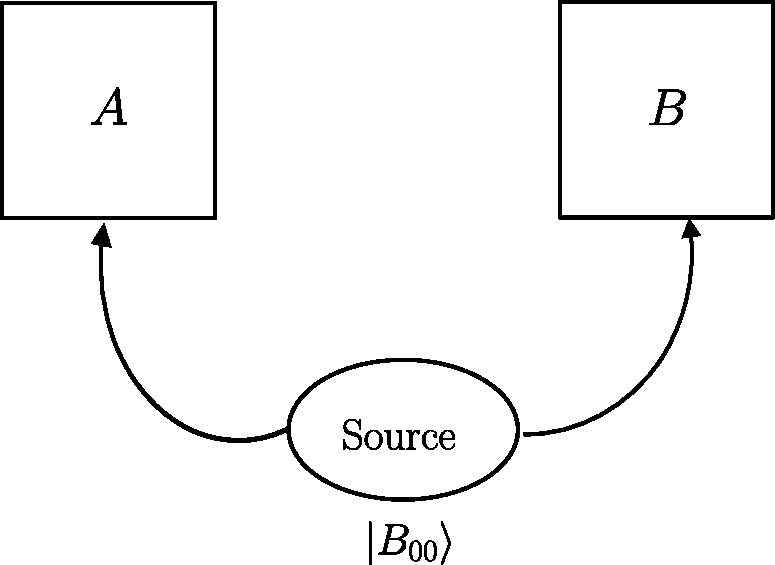
\includegraphics[width=0.5\textwidth]{figures/2026-10-14_2.pdf}
\caption{Ekert protocol}
\end{figure}


\begin{itemize}
    \item Alice and Bob keep secret the basis in which they will do the measurement and have either $0$ or $1$ giving $x_i = 0, 1$ and $y_i = 0, 1$.
\end{itemize}
Alice will have the angles
\begin{align*} 
	\alpha_1 &=  -\frac{\pi}{4} \\
	\alpha_2 &= - \frac{\pi}{8}\\
	\alpha_3 &= 0
\end{align*}
Bob will have 
\begin{align*} 
	\beta_1 &=  -\frac{\pi}{8} \\
	 \beta_2 &=  0\\
	 \beta_3 &= -\frac{\pi}{8}
\end{align*}

Alice and Bob reveal the basis choices for the angles $\alpha_1, \alpha_3, \beta_1, \beta_3$. They compute $X^{\text{experimental}}=  2 \sqrt{2}$ which is correct only if there is no eavesdropper. We can then produce an OTP by taking bits for angles 
\begin{align*} 
	\left(\alpha_2, \beta_1\right) &= \left(-\frac{\pi}{8}, - \frac{\pi}{8}\right) \\
	\text{and }\left(\alpha_3, \beta_2\right) &= \left(0, 0\right)
\end{align*}
In which we have $x_i = y_i$.




















